%!TEX program = xelatex
\documentclass[12pt,a4paper]{article}
\usepackage{ctex}
\usepackage{amsmath,amscd,amsbsy,amssymb,latexsym,url,bm,amsthm}
\usepackage{epsfig,graphicx,subfigure}
\usepackage{enumitem,balance,mathtools}
\usepackage{wrapfig}
\usepackage{mathrsfs, euscript}
\usepackage[usenames]{xcolor}
\usepackage{hyperref}
\usepackage{float}
%\usepackage{algorithm}
%\usepackage{algorithmic}
%\usepackage[vlined,ruled,commentsnumbered,linesnumbered]{algorithm2e}
\usepackage[ruled,lined,boxed,linesnumbered]{algorithm2e}

\newtheorem{theorem}{Theorem}[section]
\newtheorem{lemma}[theorem]{Lemma}
\newtheorem{proposition}[theorem]{Proposition}
\newtheorem{corollary}[theorem]{Corollary}
\newtheorem{exercise}{Exercise}[section]
\newtheorem*{solution}{Solution}

\renewcommand{\thefootnote}{\fnsymbol{footnote}}

\newcommand{\postscript}[2]
 {\setlength{\epsfxsize}{#2\hsize}
  \centerline{\epsfbox{#1}}}

\renewcommand{\baselinestretch}{1.0}

\setlength{\oddsidemargin}{-0.365in}
\setlength{\evensidemargin}{-0.365in}
\setlength{\topmargin}{-0.3in}
\setlength{\headheight}{0in}
\setlength{\headsep}{0in}
\setlength{\textheight}{10.1in}
\setlength{\textwidth}{7in}
\makeatletter \renewenvironment{proof}[1][Proof] {\par\pushQED{\qed}\normalfont\topsep6\p@\@plus6\p@\relax\trivlist\item[\hskip\labelsep\bfseries#1\@addpunct{.}]\ignorespaces}{\popQED\endtrivlist\@endpefalse} \makeatother
\makeatletter
\renewenvironment{solution}[1][Solution] {\par\pushQED{\qed}\normalfont\topsep6\p@\@plus6\p@\relax\trivlist\item[\hskip\labelsep\bfseries#1\@addpunct{.}]\ignorespaces}{\popQED\endtrivlist\@endpefalse} \makeatother
\begin{document}
\noindent

%========================================================================
\noindent\framebox[\linewidth]{\shortstack[c]{
\Large{\textbf{CS308 Homework 1}}\vspace{1mm}\\
Exercises for Algorithm Design and Analysis by Li Jiang, 2016 Autumn Semester}}
\begin{center}
\footnotesize{\color{blue} \quad Name:\underline {Gao Chao}  \quad Student ID:\underline {5142029014} \quad Email: \underline {gaoc96@163.com} }
\end{center}

\begin{description}
	\item[Coverage]: This assginment covers the chapter 3.7 incluing coverting NFA to DFA, regular expression to DFA and transition table.
\end{description}

\begin{enumerate}
\item (Section 3.7, Exercises 3.7.1) Convert to DFA's the NFA's of:

    \begin{enumerate}
    \item Fig. 3.26.

    \begin{figure}[h]
    \center
    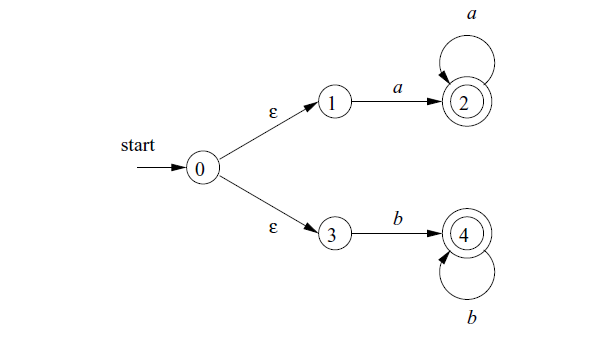
\includegraphics[width=0.8\linewidth]{Fig3-26}\vspace{-10pt}
    \caption{Fig. 3.26.} \label{fig:3.26}\vspace{-10pt}
    \end{figure}

    \textrm{\\}
    \textrm{\\}

    \item Fig. 3.29.

    \begin{figure}[h]
    \center
    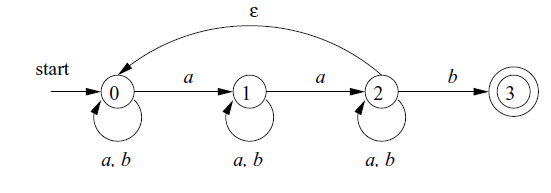
\includegraphics[width=0.8\linewidth]{Fig3-29}\vspace{-10pt}
    \caption{Fig. 3.29.} \label{fig:3.29}\vspace{-10pt}
    \end{figure}

    \newpage

    \item Fig. 3.30.

    \begin{figure}[h]
    \center
    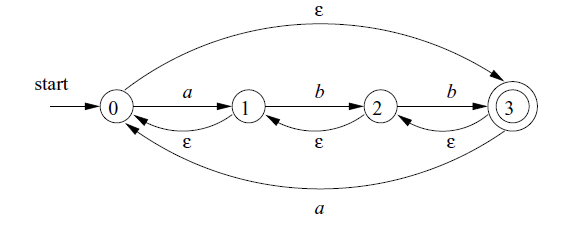
\includegraphics[width=0.8\linewidth]{Fig3-30}\vspace{-10pt}
    \caption{Fig. 3.30.} \label{fig:3.30}\vspace{-10pt}
    \end{figure}

    \end{enumerate}

%\begin{solution}
    \textrm{\\}
    \begin{enumerate}
    \item solution of a
    \begin{table}[h]
    \centering
    \begin{tabular}{|c|c|c|c|}
    \hline
    NFA state & DFA state & a & b\\
    \hline
    \{ 0, 1, 3 \} & A & B & C\\
    \hline
    \{ 2 \} & B & B & $\varnothing$\\
    \hline
    \{ 4 \} & C & $\varnothing$ & C\\
    \hline
    \end{tabular}
    \caption{transition table}
    \end{table}

    \begin{figure}[h]
    \center
    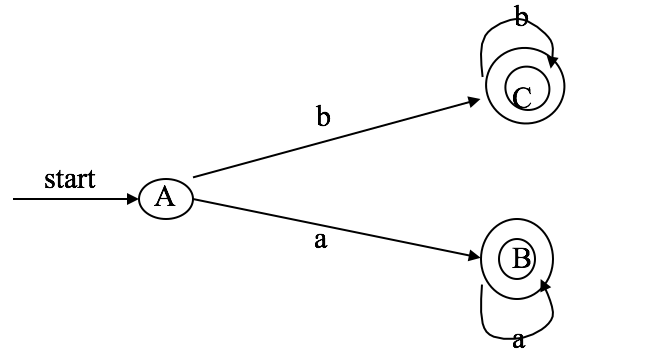
\includegraphics[width=0.8\linewidth]{sol1}\vspace{-10pt}
    \caption{DFA} \label{DFA}\vspace{-10pt}
    \end{figure}
    
    \newpage
    \textrm{\\}
    \textrm{\\}
    \item solution of b
    \textrm{\\}
    \begin{table}[h]
    \centering
    \begin{tabular}{|c|c|c|c|}
    \hline
    NFA state & DFA state & a & b\\
    \hline
    \{ 0 \} & A & B & A\\
    \hline
    \{ 0, 1 \} & B & C & B\\
    \hline
    \{ 0, 1, 2 \} & C & C & D\\
    \hline
    \{ 0, 1, 2, 3 \} & D & C & D\\
    \hline
    \end{tabular}
    \caption{transition table}
    \end{table}

    \textrm{\\}
    \textrm{\\}
    \begin{figure}[h]
    \center
    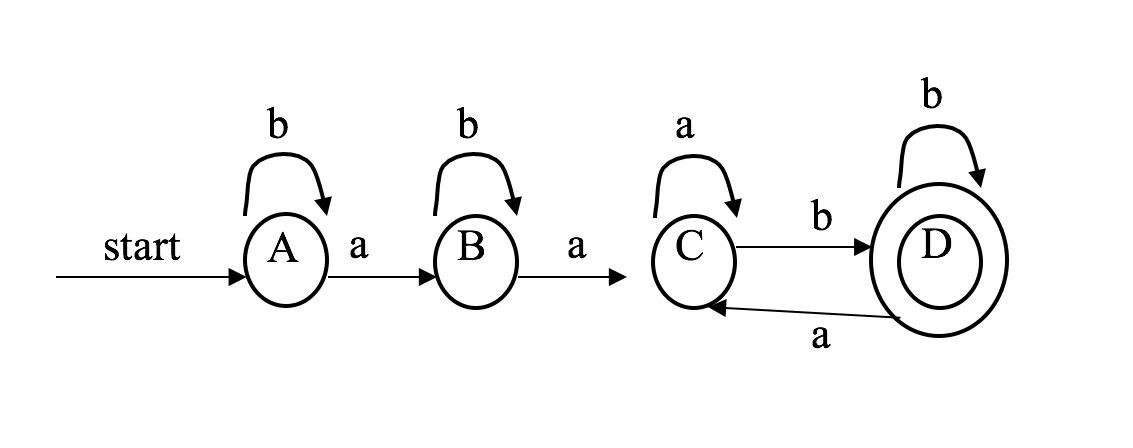
\includegraphics[width=0.8\linewidth]{sol2}\vspace{-10pt}
    \caption{DFA} \label{DFA}\vspace{-10pt}
    \end{figure}

    \newpage
    \textrm{\\}
    \textrm{\\}
    \item solution of c
    \textrm{\\}
    \begin{table}[h]
    \centering
    \begin{tabular}{|c|c|c|c|}
    \hline
    NFA state & DFA state & a & b\\
    \hline
    \{ 0, 1, 2, 3 \} & A & A & A\\
    \hline
    \end{tabular}
    \caption{transition table}
    \end{table}

    \textrm{\\}
    \textrm{\\}
    \begin{figure}[h]
    \center
    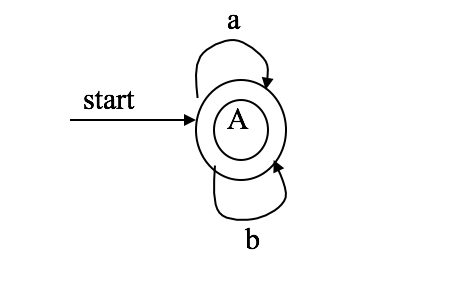
\includegraphics[width=0.8\linewidth]{sol3}\vspace{-10pt}
    \caption{DFA} \label{DFA}\vspace{-10pt}
    \end{figure}

    \end{enumerate}
%Your answer should be written here.

%\end{solution}
\newpage
\textrm{\\}

\item (Section 3.7, Exercises 3.7.2) use Algorithm 3.22 to simulate the NFA's on input \emph{aabb} regarding the above Fig 3.29 and Fig 3.30.

    \textbf{Algorithm 3.22:}

    \textbf{INPUT}: An input string $x$ terminated by an end-of-file character eof. An NFA $N$ with start state $s_0$, accepting states $F$, and transition function move.

    \textbf{OUTPUT}: Answer ''yes'' if $N$ accepts $x$. Answer ''no'' otherwise.

    \textbf{EXAMPLE}: $-start->\{0\}-a->\{0,1\}-a->\{0,1,2\}-b->\{0,2,3\}-b->\{0,2,3\}$


%\begin{solution}
    \textrm{\\}
    \textbf{Solutions}:
    \textrm{\\}
    1. $-start->\{0\}-a->\{0,1\}-a->\{0,1,2\}-b->\{0,1,2,3\}-b->\{0,1,2,3\}$
    \newline2. $-start->\{0,1,2,3\}-a->\{0,1,2,3\}-a->\{0,1,2,3\}-b->\{0,1,2,3\}-b->\{0,1,2,3\}$
%Your answer should be written here.

%\end{solution}

\textrm{\\}

\item (Section 3.7, Exercises 3.7.3) Convert the following regular expressions to deterministic finite automata, using algorithms 3.23 and 3.20:

    \textbf{Algorithm 3.20}:

    \textbf{INPUT}: An NFA $N$.

    \textbf{OUTPUT}:A DFA $D$ accepting the same language as $N$.

    \textrm{\\}

    \textbf{Algorithm 3.23}:

    \textbf{INPUT}:A regular expression $r$ over alphabet $\sum$.

    \textbf{OUTPUT}: An NFA $N$ accepting $L(r)$.

    \begin{enumerate}
    \item $(a|b)^*$
    \item $(a^*|b^*)^*$
    \item $((\varepsilon|a)|b^*)^*$
    \end{enumerate}

    \newpage

    \textbf{EXAMPLE}:
    \begin{figure}[h]
    \center
    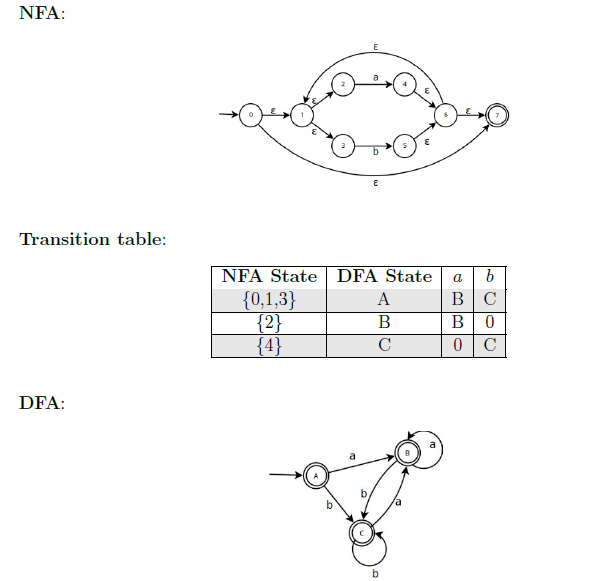
\includegraphics[width=0.8\linewidth]{Example}\vspace{-10pt}
    \caption{An example.} \label{fig:example}\vspace{-10pt}
    \end{figure}


%\begin{solution}
    \newpage
    \textbf{Solutions}:
    \begin{enumerate}
    \item $(a|b)^*$
    \textrm{\\}
    \begin{figure}[h]
    \center
    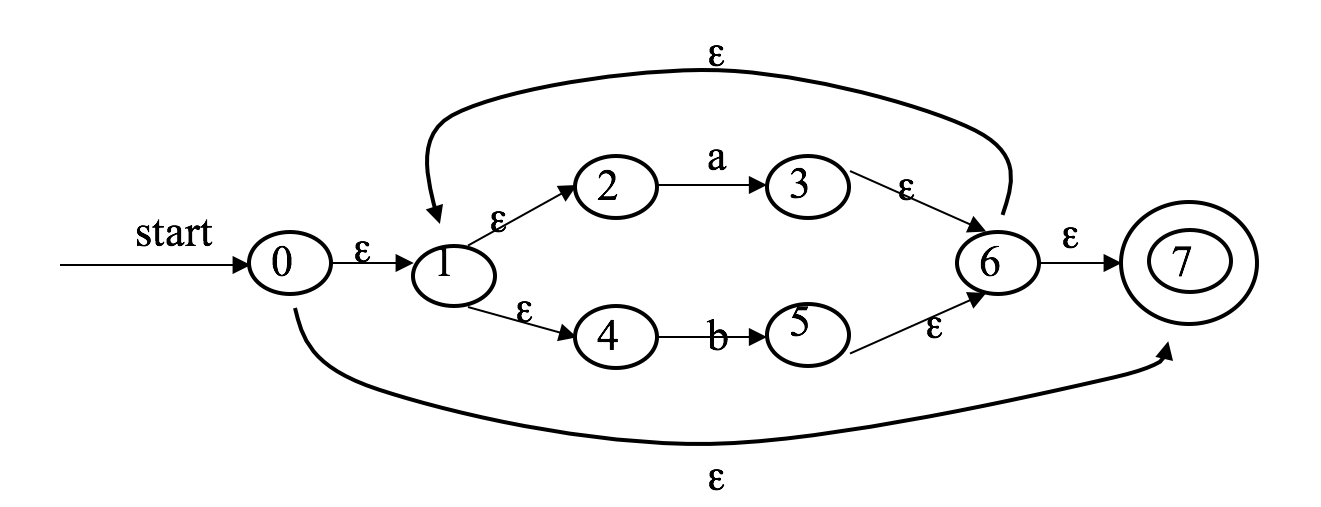
\includegraphics[width=0.8\linewidth]{sol4}\vspace{-10pt}
    \caption{NFA} \label{NFA}\vspace{-10pt}
    \end{figure}

    \textrm{\\}
    \begin{table}[h]
    \centering
    \begin{tabular}{|c|c|c|c|}
    \hline
    NFA state & DFA state & a & b\\
    \hline
    \{ 0, 1, 2, 4, 7 \} & A & B & C\\
    \hline
    \{ 1, 2, 3, 4, 6, 7 \} & B & B & C\\
    \hline
    \{ 1, 2, 4, 5, 6, 7 \} & C & B & C\\
    \hline
    \end{tabular}
    \caption{transition table}
    \end{table}

    \textrm{\\}
    \begin{figure}[h]
    \center
    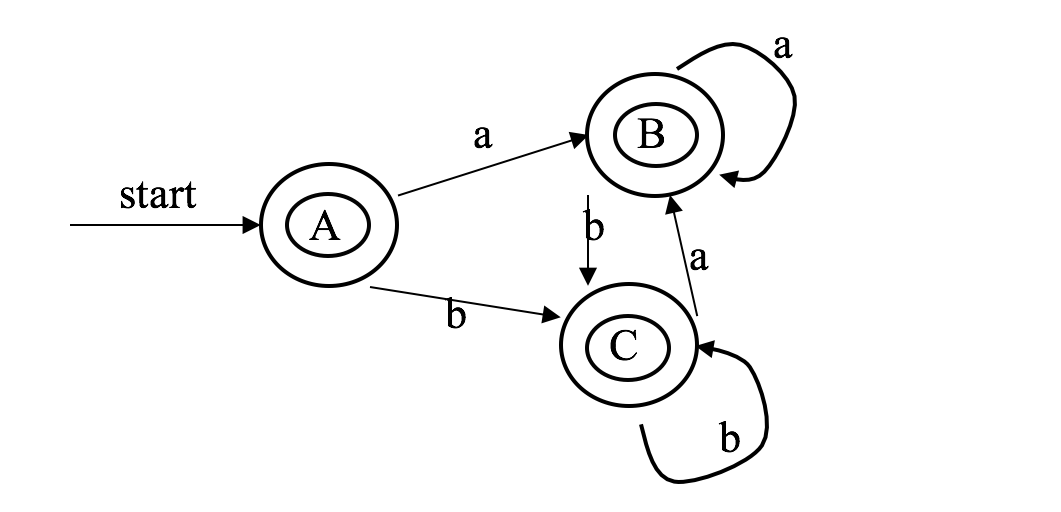
\includegraphics[width=0.8\linewidth]{sol5}\vspace{-10pt}
    \caption{DFA} \label{DFA}\vspace{-10pt}
    \end{figure}

    \newpage
    \item $(a^*|b^*)^*$
    \textrm{\\}
    \begin{figure}[h]
    \center
    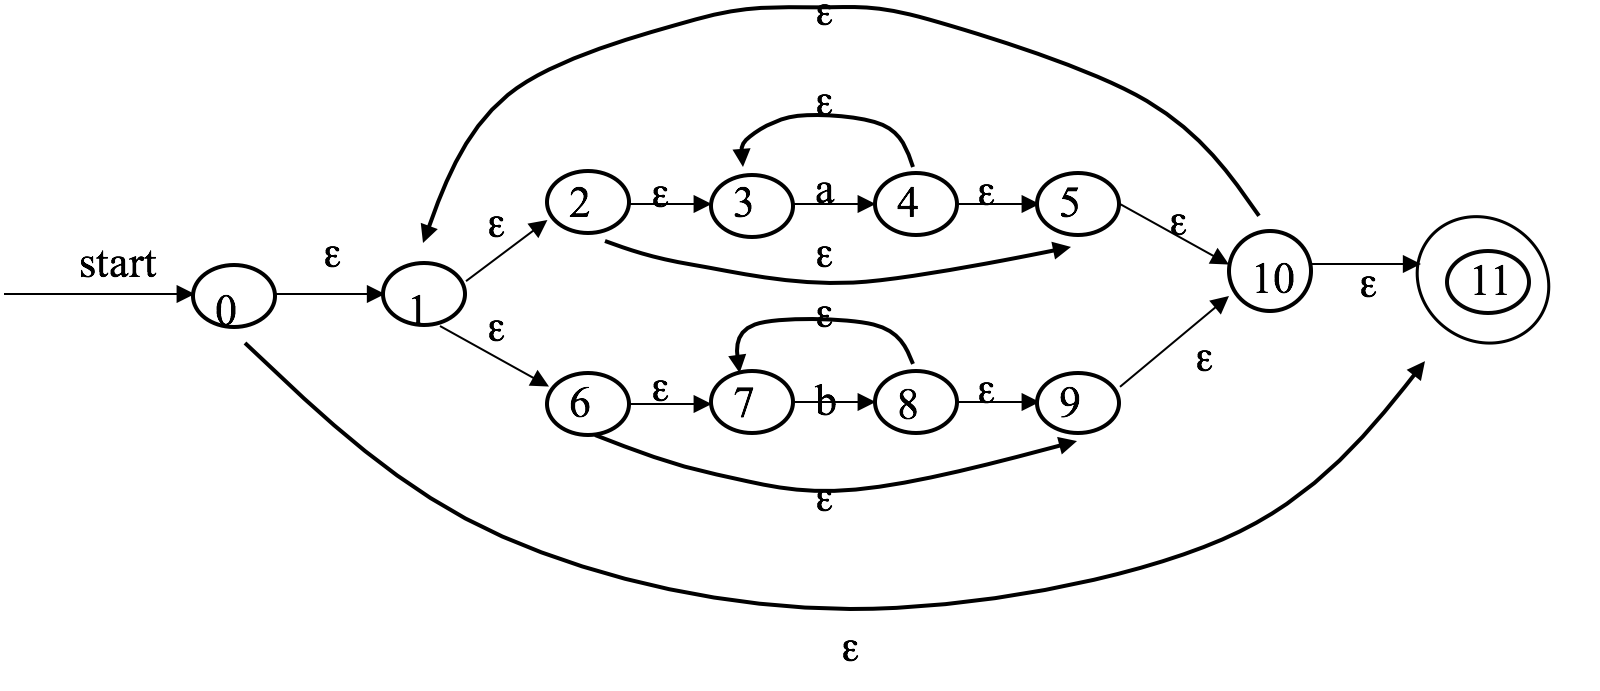
\includegraphics[width=0.8\linewidth]{sol6}\vspace{-10pt}
    \caption{NFA} \label{NFA}\vspace{-10pt}
    \end{figure}

    \textrm{\\}
    \begin{table}[h]
    \centering
    \begin{tabular}{|c|c|c|c|}
    \hline
    NFA state & DFA state & a & b\\
    \hline
    \{ 0, 1, 2, 3, 5, 6 ,7, 9, 10, 11 \} & A & B & C\\
    \hline
    \{ 1, 2, 3, 4, 5, 6, 7, 9, 10, 11 \} & B & B & C\\
    \hline
    \{ 1, 2, 3, 5, 6, 7, 8, 9, 10, 11 \} & C & B & C\\
    \hline
    \end{tabular}
    \caption{transition table}
    \end{table}

    \textrm{\\}
    \begin{figure}[h]
    \center
    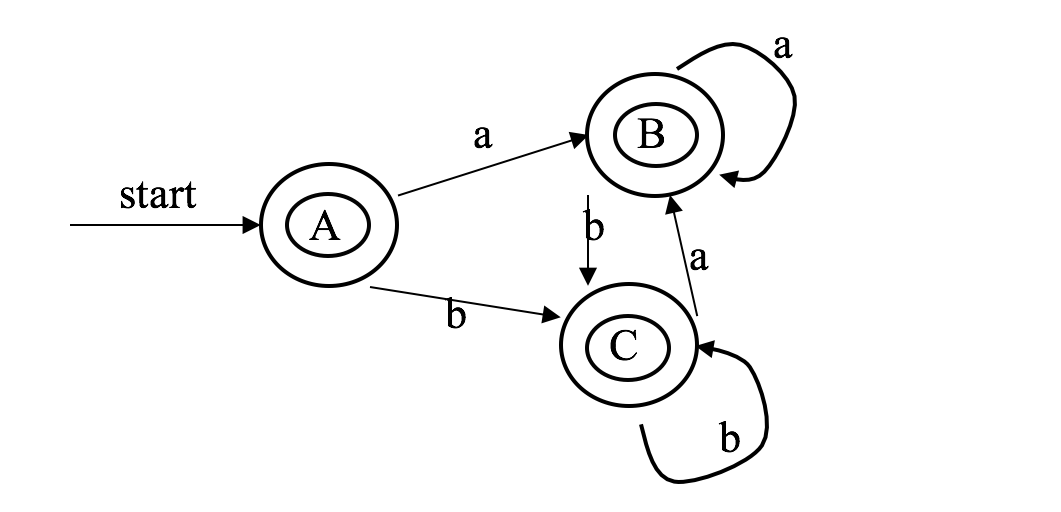
\includegraphics[width=0.8\linewidth]{sol5}\vspace{-10pt}
    \caption{DFA} \label{DFA}\vspace{-10pt}
    \end{figure}

    \newpage
    \item $((\varepsilon|a)|b^*)^*$
    \textrm{\\}
    \begin{figure}[h]
    \center
    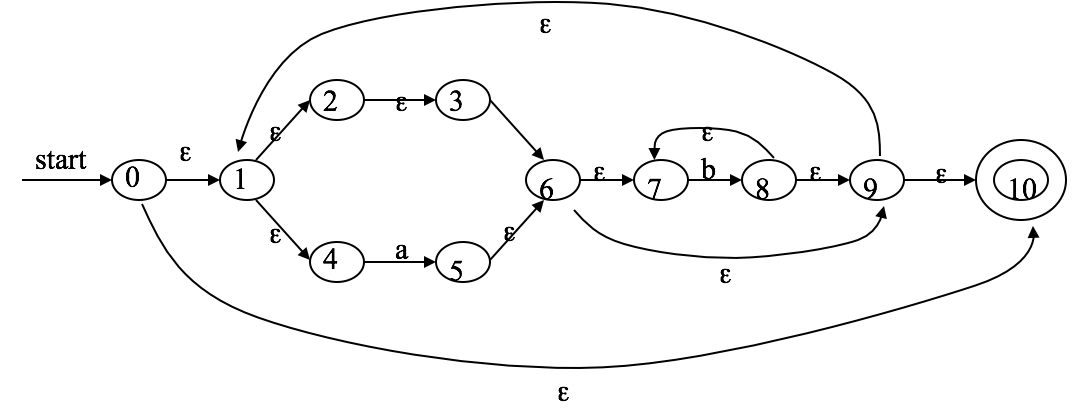
\includegraphics[width=0.8\linewidth]{sol7}\vspace{-10pt}
    \caption{NFA} \label{NFA}\vspace{-10pt}
    \end{figure}

    \textrm{\\}
    \begin{table}[h]
    \centering
    \begin{tabular}{|c|c|c|c|}
    \hline
    NFA state & DFA state & a & b\\
    \hline
    \{ 0, 1, 2, 3, 4, 6 ,7, 9, 10 \} & A & B & C\\
    \hline
    \{ 1, 2, 3, 4, 5, 6, 7, 9, 10 \} & B & B & C\\
    \hline
    \{ 1, 2, 3, 4, 6, 7, 8, 9, 10 \} & C & B & C\\
    \hline
    \end{tabular}
    \caption{transition table}
    \end{table}

    \textrm{\\}
    \begin{figure}[h]
    \center
    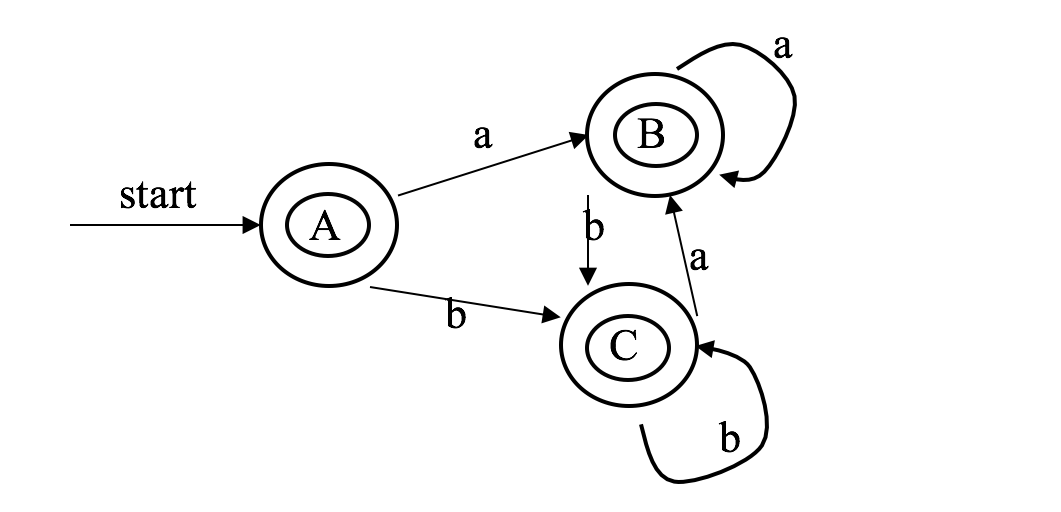
\includegraphics[width=0.8\linewidth]{sol5}\vspace{-10pt}
    \caption{DFA} \label{DFA}\vspace{-10pt}
    \end{figure}

    \end{enumerate}
%Your answer should be written here.

%\end{solution}



\end{enumerate}
%========================================================================
\end{document}
